% Copyright (C) 2014-2017 by Thomas Auzinger <thomas@auzinger.name>

\documentclass[draft,final]{vutinfth} % Remove option 'final' to obtain debug information.

% Load packages to allow in- and output of non-ASCII characters.
\usepackage{lmodern}        % Use an extension of the original Computer Modern font to minimize the use of bitmapped letters.
\usepackage[T1]{fontenc}    % Determines font encoding of the output. Font packages have to be included before this line.
\usepackage[utf8]{inputenc} % Determines encoding of the input. All input files have to use UTF8 encoding.

% Extended LaTeX functionality is enables by including packages with \usepackage{...}.
\usepackage{amsmath}    % Extended typesetting of mathematical expression.
\usepackage{amssymb}    % Provides a multitude of mathematical symbols.
\usepackage{mathtools}  % Further extensions of mathematical typesetting.
\usepackage{microtype}  % Small-scale typographic enhancements.
\usepackage[inline]{enumitem} % User control over the layout of lists (itemize, enumerate, description).
\usepackage{multirow}   % Allows table elements to span several rows.
\usepackage{booktabs}   % Improves the typesettings of tables.
\usepackage{subcaption} % Allows the use of subfigures and enables their referencing.
\usepackage[ruled,linesnumbered,algochapter]{algorithm2e} % Enables the writing of pseudo code.
\usepackage[usenames,dvipsnames,table]{xcolor} % Allows the definition and use of colors. This package has to be included before tikz.
\usepackage{nag}       % Issues warnings when best practices in writing LaTeX documents are violated.
\usepackage{todonotes} % Provides tooltip-like todo notes.
\usepackage{hyperref}  % Enables cross linking in the electronic document version. This package has to be included second to last.
\usepackage[acronym,toc]{glossaries} % Enables the generation of glossaries and lists fo acronyms. This package has to be included last.
\usepackage{paralist} %Allows usage of inline lists

% Define convenience functions to use the author name and the thesis title in the PDF document properties.
\newcommand{\authorname}{Stefan Gamerith} % The author name without titles.
\newcommand{\thesistitle}{Enrichment of Crowdsourcing Tasks with Contextual Data} % The title of the thesis. The English version should be used, if it exists.

% Set PDF document properties
\hypersetup{
    pdfpagelayout   = TwoPageRight,           % How the document is shown in PDF viewers (optional).
    linkbordercolor = {Melon},                % The color of the borders of boxes around crosslinks (optional).
    pdfauthor       = {\authorname},          % The author's name in the document properties (optional).
    pdftitle        = {\thesistitle},         % The document's title in the document properties (optional).
    pdfsubject      = {Subject},              % The document's subject in the document properties (optional).
    pdfkeywords     = {a, list, of, keywords} % The document's keywords in the document properties (optional).
}

\setpnumwidth{2.5em}        % Avoid overfull hboxes in the table of contents (see memoir manual).
\setsecnumdepth{subsection} % Enumerate subsections.

\nonzeroparskip             % Create space between paragraphs (optional).
\setlength{\parindent}{0pt} % Remove paragraph identation (optional).

\makeindex      % Use an optional index.
\makeglossaries % Use an optional glossary.
%\glstocfalse   % Remove the glossaries from the table of contents.

% Set persons with 4 arguments:
%  {title before name}{name}{title after name}{gender}
%  where both titles are optional (i.e. can be given as empty brackets {}).
\setauthor{}{\authorname}{BSc.}{male}
\setadvisor{}{Reka Marta Sabou}{MSc., PhD}{female}

% For bachelor and master theses:
%\setfirstassistant{Pretitle}{Forename Surname}{Posttitle}{male}
%\setsecondassistant{Pretitle}{Forename Surname}{Posttitle}{male}
%\setthirdassistant{Pretitle}{Forename Surname}{Posttitle}{male}

% For dissertations:
%\setfirstreviewer{Pretitle}{Forename Surname}{Posttitle}{male}
%\setsecondreviewer{Pretitle}{Forename Surname}{Posttitle}{male}

% For dissertations at the PhD School and optionally for dissertations:
% \setsecondadvisor{Pretitle}{Forename Surname}{Posttitle}{male} % Comment to remove.

% Required data.
\setaddress{Linzerstrasse 429/4215, 1140 Wien}
\setregnumber{0925081}
\setdate{01}{01}{2001} % Set date with 3 arguments: {day}{month}{year}.
\settitle{\thesistitle}{\thesistitle} % Sets English and German version of the title (both can be English or German). If your title contains commas, enclose it with additional curvy brackets (i.e., {{your title}}) or define it as a macro as done with \thesistitle.
%\setsubtitle{Optional Subtitle of the Thesis}{Optionaler Untertitel der Arbeit} % Sets English and German version of the subtitle (both can be English or German).

% Select the thesis type: bachelor / master / doctor / phd-school.
% Bachelor:
%\setthesis{bachelor}
%
% Master:
\setthesis{master}
\setmasterdegree{dipl.} % dipl. / rer.nat. / rer.soc.oec. / master
%
% Doctor:
%\setthesis{doctor}
%\setdoctordegree{rer.soc.oec.}% rer.nat. / techn. / rer.soc.oec.
%
% Doctor at the PhD School
%\setthesis{phd-school} % Deactivate non-English title pages (see below)

% For bachelor and master:
\setcurriculum{Software Engineering / Internet Computing}{Software Engineering / Internet Computing} % Sets the English and German name of the curriculum.

% For dissertations at the PhD School:
%\setfirstreviewerdata{Affiliation, Country}
%\setsecondreviewerdata{Affiliation, Country}


\begin{document}

\frontmatter % Switches to roman numbering.
% The structure of the thesis has to conform to
%  http://www.informatik.tuwien.ac.at/dekanat

\addtitlepage{naustrian} % German title page (not for dissertations at the PhD School).
\addtitlepage{english} % English title page.
\addstatementpage

\begin{danksagung*}
\todo{Ihr Text hier.}
\end{danksagung*}

\begin{acknowledgements*}
\todo{Enter your text here.}
\end{acknowledgements*}

\begin{kurzfassung}
\todo{Ihr Text hier.}
\end{kurzfassung}

\begin{abstract}
\todo{Enter your text here.}
\end{abstract}

% Select the language of the thesis, e.g., english or naustrian.
\selectlanguage{english}

% Add a table of contents (toc).
\tableofcontents % Starred version, i.e., \tableofcontents*, removes the self-entry.

% Switch to arabic numbering and start the enumeration of chapters in the table of content.
\mainmatter



\chapter{Introduction}
\todo{Enter your text here.}
\section{Motivation}
\todo{Enter your text here.}
\section{Aim of the Work (e.g. Research Questions)}
\todo{Enter your text here.}
\section{Contributions}
\todo{Enter your text here.}
\section{Structure of the Work}
\todo{Enter your text here.}



\chapter{State of the Art}
\todo{Enter your text here.}
\section{Crowdsourcing}
\todo{Enter your text here.}
\section{Crowdsourcing in the Semantic Web}
\todo{Enter your text here.}
\section{The uComp Protege Plugin}
\todo{Enter your text here.}
\section{Enrichment of crowdsourcing tasks with contextual data}
\todo{Enter your text here.}



\chapter{Methodology}
\todo{Enter your text here.}



\chapter{Context Enrichment Methods}\label{chap:context_enrichment_methods}
While in~\hyperref[chap:implementation]{Chapter~\ref*{chap:implementation}} the technical foundation for implementing the Context Enrichment Methods was built, this Chapter describes these on a more conceptual level. There was no limitation on the used settings or data. Instead, the context used for ontology validation was created from general purpose internal and external sources. 

First, \hyperref[sec:neighboring_nodes]{Section~\ref*{sec:neighboring_nodes}} introduces a novel Context Enrichment Method which takes neighboring nodes~(i.e. subclass relations) into account. Second, a method of embedded context using metadata is discussed in \hyperref[sec:embedded_context]{Section~\ref*{sec:embedded_context}} and last, \hyperref[sec:external_source]{Section~\ref*{sec:external_source}} contains Context Enrichment using data from external sources.
\section{Neighboring Nodes}\label{sec:neighboring_nodes}
This Section starts with an conceptual overview of how neighboring nodes in an ontology graph are used to generate contextual information for ontology validation. Then, existing approaches on generating textual definitions for an ontology are examined. As in the literature~\cite{soton265735} the term \textit{ontology verbalisation} is commonly used as a short-term for that task, it is used in the remainder of this Section. We conclude that even though that there exists the major tool \textit{OWL Verbalizer}\footnote{\url{http://mcs.open.ac.uk/nlg/SWAT/Verbaliser.html} accessed 2018/04/30} which transforms a generic OWL~ontology into english sentences, we could not integrate it into Context Enrichment process because 
\begin{inparaenum}[a)]
		\item it was designed as a standalone tool written in SWI-Prolog\footnote{\url{http://www.swi-prolog.org/} accessed 2018/04/30} and
		\item as input it only accepts the whole OWL~ontology 
\end{inparaenum}.
However, to make concept definitions and relations more understandable for non-experts, some revised rules were integrated in our enrichment process.

To illustrate the concept of neighboring nodes and how they relate to the Context Enrichment approach explained later, a simple ontology graph is given in~\hyperref[fig:simple_owl_graph]{Figure~\ref*{fig:simple_owl_graph}} describing the teacher/pupil domain.
\begin{figure}
	 \centering
	 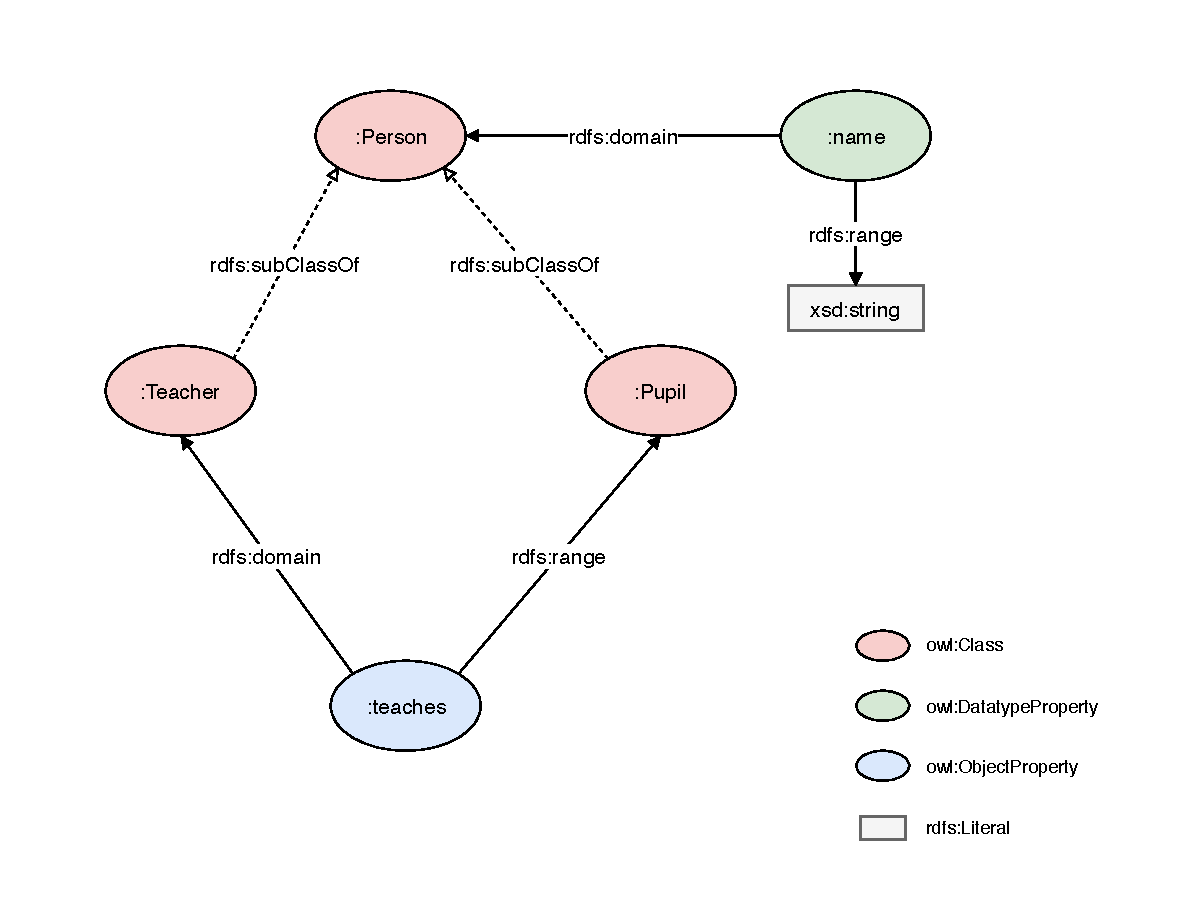
\includegraphics[width=\textwidth]{drawio/University_Ontology_Example}
	 \caption{Simple OWL ontology graph}\label{fig:simple_owl_graph}
\end{figure}
For example, if the concept \textit{:Teacher} is taken as reference node, it makes sense to not only consider the concept itself, but instead include connected nodes~(e.g. the concept \textit{:Person} and the object property \textit{:teaches}) in the enrichment process. 

As in the guidelines for conducting crowdsourcing research~\cite{sarasua2015crowdsourcing}, the authors recommended to avoid technical terms in crowdsourcing questions. To facilitate this need, we examined an existing approach on ontology verbalisation and how they could be integrated in the Context Enrichment process. 

Despite the fact that natural language is desirable for descriptions as everybody knows and understands it with no extra learning effort, it conflicts with highly expressive, domain specific and formal knowledge representations. Formally specified ontologies on the other hand facilitate encoding complex relations in domain-specific areas. To resolve this conflict, the new language variant \textbf{ACE}~\textit{(Attempto Controlled English)}~\cite{fuchs2008} was proposed. ACE is a formal language, capable of expressing domain-specific knowledge with a well-defined syntax, supporting formal reasoning and readable by specialists who are yet unfamiliar with formal languages and methods.

As our approach described later in this section is based on ACE\footnote{\url{https://tinyurl.com/yc3zhu9a} accessed 2018/05/05}\footnote{\url{https://tinyurl.com/ycst39jv} accessed 2018/05/05}, a short overview of ACE' language structure is given in the following paragraphs:
 
 \paragraph{Simple Sentences} A Simple Sentence derived from standard English contains a subject and a verb: \texttt{subject + verb + complements [ + adjuncts ]} In addition the verb relate direct or indirect to one or more other objects~(\textit{complements}). Optionally, to add more specificity one or more adverbs and prepositional phrases can be added~(\textit{adjuncts}). 

\paragraph{Composite Sentences} A Composite Sentence is recursively built from one or more Simple Sentences connected by \textit{coordination},
\textit{subordination}, \textit{quantification} and \textit{negation}. Whereas, coordination is associates sentences either by the word \texttt{and} or \texttt{or}, subordination describes dependent sentences in some form of relation to each other~(e.g. if-then sentences). Quantification enables expressing statements about all~(universal quantification) or certain~(existential quantification) objects of a certain domain. Last, negation is a way encode negative polarity in a sentence~(e.g. sentences containing \texttt{not} or \texttt{no}). 

\paragraph{Query Sentences} Query Sentences can be divided into polar questions~(e.g. with \textit{yes/no} answer) and non-polar questions, also known as \emph{wh-questions}. For those there does not exist a pre-defined answer, as in contrast to the former yes/no questions. Furthermore, wh-questions start with either of the following five W-words: \texttt{Who}, \texttt{What}, \texttt{When}, \texttt{Where} and \texttt{Why}. However, sometimes questions starting with the word \texttt{How} are added to the category of wh-questions.

\paragraph{Anaphoric References} In case the meaning of a word or phrase depends on the context, multiple occurrences of these expressions are called \textit{Anaphoric References}. More specifically, the referring term~(\textit{anaphor}) relates to an antecedent expression. For example in the sentence \texttt{Tom arrived, but nobody noticed him}, the pronoun \texttt{him} relates to \texttt{Tom}. To resolve ambiguities during the processing phase, Anaphoric References are replaced by encoded references. 

Among others, one application areas of ACE is \textbf{OWL Verbalizer}~\cite{stevens2011}, an open source tool aiming at producing ACE texts from generic OWL ontologies. A description on the major concepts of OWL Verbaliser where our approach is based on is given below:

To overcome the burden of manual authoring ontology definitions, the tool formally known as OWL Verbaliser and now part of the \textbf{SWAT Tool Suite}\footnote{\url{http://mcs.open.ac.uk/nlg/SWAT/} accessed 2018/05/06} was created. Whereas producing high quality texts in restricted application domains is an active research field, this tool aims at generating understandable und useful descriptions that are of moderate quality using general-purpose methods.

The high-level process of ontology verbalization depicted from \hyperref[fig:verbaliser_architecture]{Figure~\ref*{fig:verbaliser_architecture}} consists of the following stages:

\paragraph{Transcoding from OWL to Prolog} Using an ontology in RDF/XML~Format as input, a file in a convenient Prolog format is generated in this
stage. The conversation process covered by the \textit{Transcoder}, \textit{Identifier~Selector} and \textit{Label~Selector} groups identifiers~(concepts, individuals, object~properties) together with labels for further processing. In addition, ambiguous terms in identifiers are standardised. 

\paragraph{Constructing a lexicon for atomic entities} The output of this stage, covered by the component \textit{Lexicon Generator}, is a collection of lexicons, computed from the normalised Prolog terms in the previous stage. A lexical entry~(lexicon) is defined as a quadruple of the following form: \texttt{<identifier, part-of-speech, singular-form, plural-form>} To facilitate processing in later stages, normalised identifiers for concepts, individuals and object~properties processed in the beginning are stored together with word category, singular form and plural form. The word~category, in linguistics also known as part-of-speech, groups words based on similar properties in terms of syntax and grammar. Common categories among others are nouns, verbs and adjectives. Last, to differentiate the quantity of described by a phrase or word, the singular and plural form of a noun is associated with each lexical entry. 
Among the storage of lexicons, the algorithm has some further rules concerning text processing implemented.  Some simple heuristics are used for pre-processing to transform the resulting word string into better readable English phrases. 

\paragraph{Selecting the axioms relevant for describing each class} This stage and next stage are covered by the \textit{Planner}.
This component has as input all axioms from the source ontology as well as the lexicons from the previous stage. In this stage axioms associated with matching lexical entries. The algorithm uses the identifier in the lexicon and the IRI~\cite{rfc3987} in ontological elements as matching criteria. 

\paragraph{Aggregating axioms with a similar structure} This stage is optional, as it is not strictly required for text generation described in the next stage. However, some improvements over using the axioms from the previous stage are achieved by grouping similar axioms. 

\paragraph{Generating sentences from axioms} The final stage is expressed by the component \textit{Realiser}, forming the central part of the
verbalisation process. English sentences are generated for each axiom using logical rules for almost every logical pattern in OWL-DL. These rules are expressed as Prolog clauses, taking the axiom and optionally the lexicon as inputs.

\begin{figure}
	 \centering
	 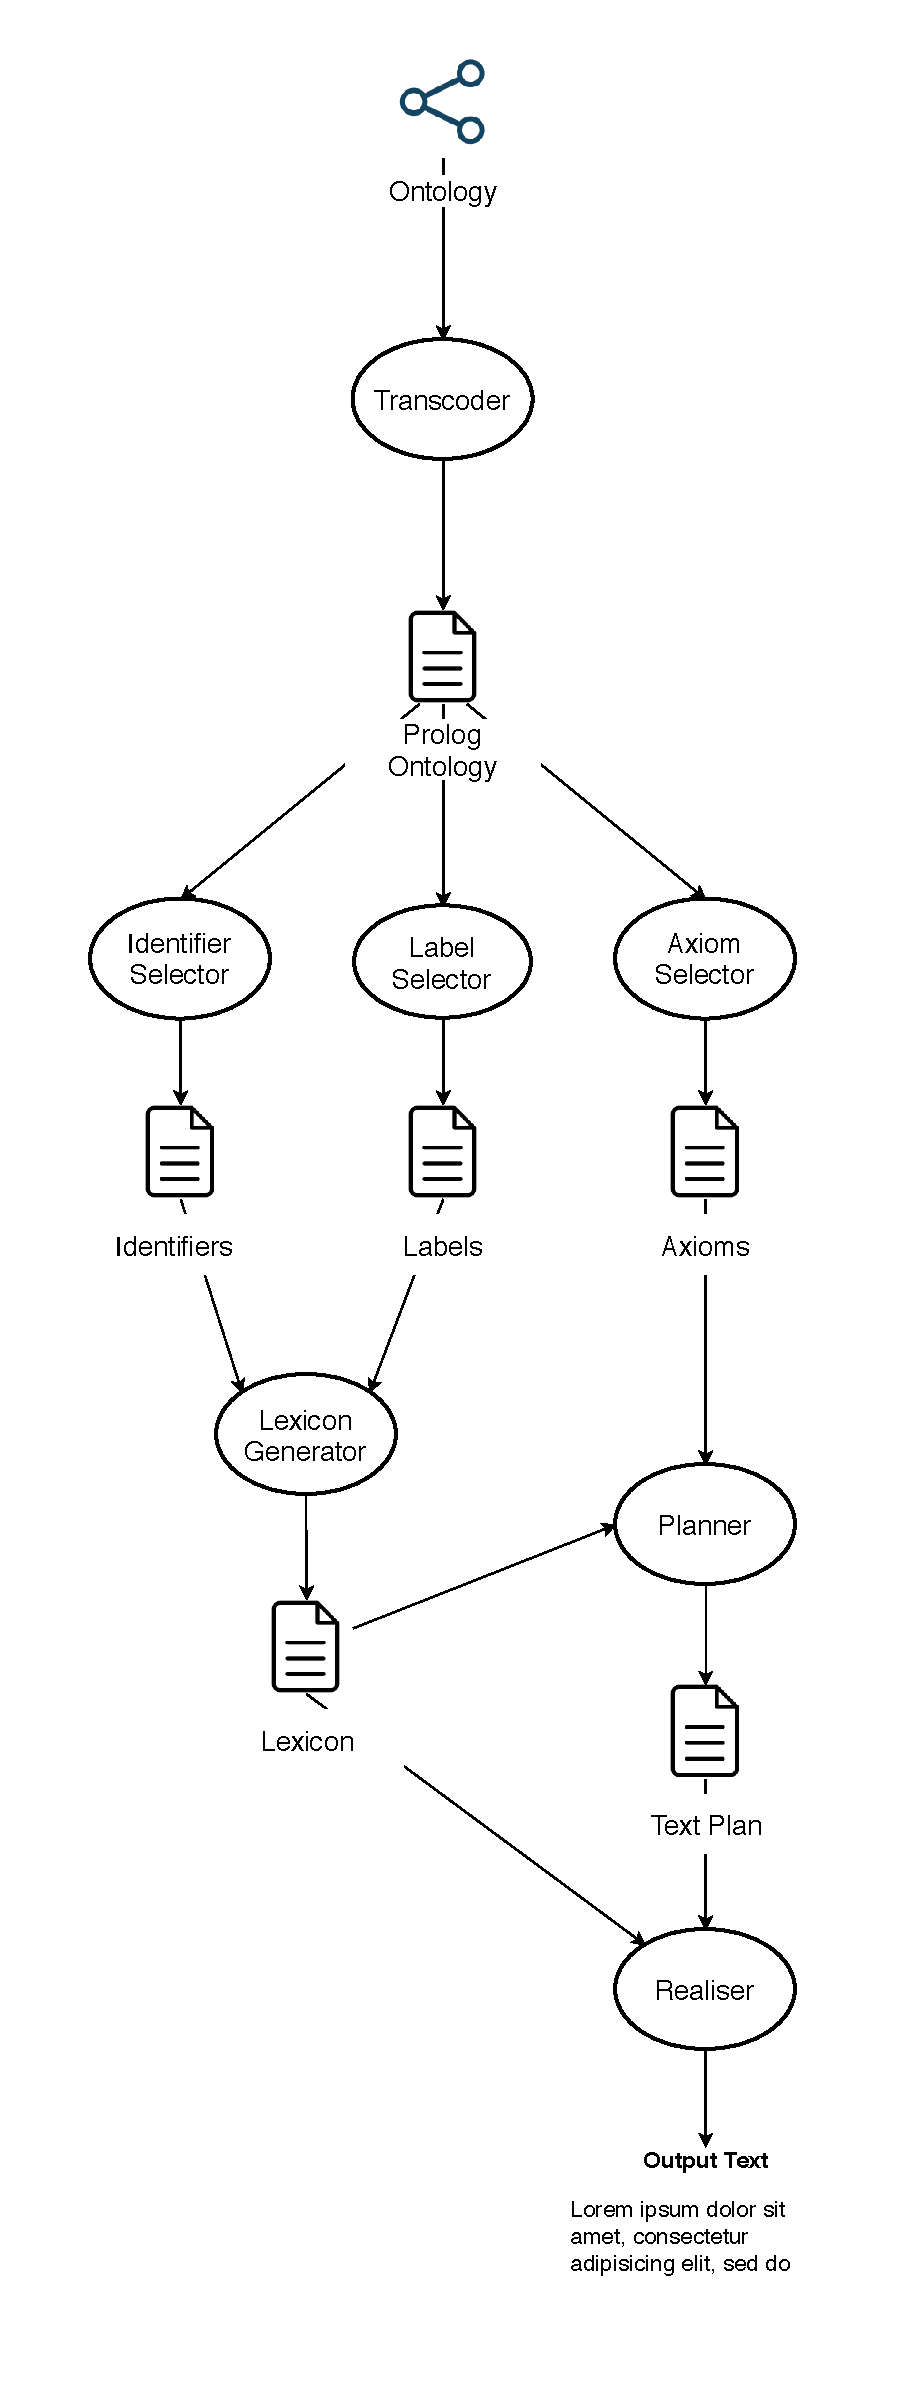
\includegraphics[width=0.5\textwidth]{drawio/Ontology_Verbaliser_Architecture}
	 \caption{Conceptual architecture of the OWL ontology verbaliser~\cite{stevens2011}}\label{fig:verbaliser_architecture}
\end{figure}


\section{Embedded Context}\label{sec:embedded_context}
%Get concept definition from wordnik
\section{External Source}\label{sec:external_source}
%On medical ontology which already has some definitions; collaboratively edited;


\chapter{Experimental Evaluation}
Initial paper~\cite{liu2005semi} for evaluation data using ontology learning techniques.
\todo{Enter your text here.}


\chapter{Implementation}\label{chap:implementation}
%Include also methods for spam detection
\section{Environment}
\section{Conceptual Architecture}




\chapter{Evaluation of the code}
\todo{Enter your text here.}
\section{Code Quality Assurance}
\todo{Enter your text here.}
\section{Background}
\todo{Enter your text here.}
\section{Quality Metrics}
\todo{Enter your text here.}
\section{Quality Evaluation}
\todo{Enter your text here.}



\chapter{Results}
\todo{Enter your text here.}



\chapter{Discussion \& Conclusion}
\todo{Enter your text here.}
%Revisit Research Questions here



\chapter{Summary \& Future Work}
\todo{Enter your text here.}



\backmatter

% Use an optional list of figures.
\listoffigures % Starred version, i.e., \listoffigures*, removes the toc entry.

% Use an optional list of tables.
\cleardoublepage % Start list of tables on the next empty right hand page.
\listoftables % Starred version, i.e., \listoftables*, removes the toc entry.

% Use an optional list of alogrithms.
%\listofalgorithms
%\addcontentsline{toc}{chapter}{List of Algorithms}

% Add an index.
%\printindex

% Add a glossary.
%\printglossaries

% Add a bibliography.
\bibliographystyle{alpha}
\bibliography{literature}

\end{document}